% =========================================================
% KHUNG TIỂU LUẬN / BÁO CÁO HỌC PHẦN — TIẾNG VIỆT
% Trình biên dịch: XeLaTeX  (BẮT BUỘC — vì dùng fontspec + polyglossia)
% Trên Overleaf: Menu → Compiler → XeLaTeX
%
% CÁCH DÙNG NHANH:
%   1. Sửa DUY NHẤT tệp  config/metadata.tex  (tên đề tài, học viên, GVHD...)
%   2. Thay logo.png bằng logo trường, figures/chuky.png bằng chữ ký
%   3. Viết nội dung trong chapters/
%   4. Biên dịch: XeLaTeX → BibTeX → XeLaTeX → XeLaTeX
% =========================================================
\documentclass[13pt]{extreport}

% =========================================================
% 1. FONT, NGÔN NGỮ
% =========================================================
\usepackage{fontspec}
% TeX Gyre Termes có cùng kích thước chữ (metric-compatible) với Times New Roman,
% dùng làm phương án dự phòng khi máy biên dịch không cài sẵn Times New Roman.
\IfFontExistsTF{Times New Roman}
  {\setmainfont{Times New Roman}}
  {\setmainfont{TeX Gyre Termes}}
\usepackage{polyglossia}
\setdefaultlanguage{vietnamese}

% =========================================================
% 2. GÓI LỆNH
% =========================================================
\usepackage{geometry}
\usepackage{setspace}
\usepackage{fancyhdr}
\usepackage{titlesec}
\usepackage{graphicx}
\usepackage{float}
\usepackage{booktabs}
\usepackage{multirow}
\usepackage{array}
\usepackage{longtable}
\usepackage{tabularx}
\usepackage{makecell}
\usepackage{caption}
\usepackage{subcaption}
\usepackage{amsmath}
\usepackage{amssymb}
% Gói algorithm/algpseudocode là tuỳ chọn (báo cáo này không dùng môi trường thuật toán).
% Chỉ nạp nếu máy biên dịch có sẵn, để tài liệu biên dịch được ngay cả khi thiếu.
\IfFileExists{algorithm.sty}{\usepackage{algorithm}}{}
\IfFileExists{algpseudocode.sty}{\usepackage{algpseudocode}}{}
\usepackage{enumitem}
\usepackage{xcolor}
\usepackage{listings}
\usepackage{url}
\usepackage[hidelinks]{hyperref}
\usepackage{indentfirst}
\usepackage{placeins}
\usepackage{tikz}
\usetikzlibrary{calc,shapes.geometric,arrows.meta,positioning,fit,backgrounds}
\usepackage{pgfplots}
\pgfplotsset{compat=1.18}
\usepgfplotslibrary{statistics}

% =========================================================
% 3. ĐỊNH DẠNG TRANG THEO QUY ĐỊNH TRƯỜNG
% =========================================================
\geometry{top=3cm,bottom=3cm,left=3cm,right=2cm}
\onehalfspacing
\setlength{\parindent}{1.25cm}
\setlength{\parskip}{0pt}

\pagestyle{fancy}
\fancyhf{}
\fancyhead[C]{\thepage}
\renewcommand{\headrulewidth}{0pt}
\renewcommand{\footrulewidth}{0pt}
\renewcommand{\normalsize}{\fontsize{13}{16}\selectfont}

% =========================================================
% 4. ĐỊNH DẠNG MÃ NGUỒN (LISTINGS)
% =========================================================
\definecolor{codegreen}{rgb}{0.0,0.55,0.0}
\definecolor{codegray}{rgb}{0.45,0.45,0.45}
\definecolor{codepurple}{rgb}{0.58,0,0.82}
\definecolor{codeback}{rgb}{0.97,0.97,0.97}

\lstdefinestyle{pystyle}{
  backgroundcolor=\color{codeback},
  commentstyle=\color{codegreen},
  keywordstyle=\color{blue},
  numberstyle=\tiny\color{codegray},
  stringstyle=\color{codepurple},
  basicstyle=\ttfamily\footnotesize,
  breakatwhitespace=false,
  breaklines=true,
  captionpos=b,
  keepspaces=true,
  numbers=left,
  numbersep=6pt,
  showspaces=false,
  showstringspaces=false,
  showtabs=false,
  tabsize=2,
  frame=single,
  rulecolor=\color{black!30}
}
\lstset{style=pystyle}

% =========================================================
% 5. THÔNG TIN ĐỀ TÀI  →  SỬA TRONG config/metadata.tex
% =========================================================
% =========================================================
%  ***  CHỈ CẦN SỬA DUY NHẤT TỆP NÀY CHO MỖI ĐỀ TÀI MỚI  ***
% =========================================================

% ---------- Trường / khoa ----------
\newcommand{\university}{TRƯỜNG ĐẠI HỌC SƯ PHẠM THÀNH PHỐ HỒ CHÍ MINH}
\newcommand{\ministry}{BỘ GIÁO DỤC VÀ ĐÀO TẠO}
\newcommand{\faculty}{Khoa Công nghệ Thông tin}

% ---------- Loại bài & học phần ----------
\newcommand{\doctype}{BÁO CÁO ĐỀ TÀI HỌC PHẦN}
\newcommand{\coursename}{(Điền tên học phần)}
\newcommand{\major}{Khoa học máy tính}
\newcommand{\courseyear}{36 (2025 -- 2027)}

% ---------- Đề tài ----------
\newcommand{\projecttitle}{Kiểm định độ tin cậy của bộ phát hiện biển báo giao thông YOLOv8 hướng-EDA}
\newcommand{\projecttitlebreak}{KIỂM ĐỊNH ĐỘ TIN CẬY CỦA BỘ PHÁT HIỆN \\ BIỂN BÁO GIAO THÔNG YOLOv8 HƯỚNG-EDA \\[6pt] {\large\mdseries\itshape Rò rỉ dữ liệu, kích thước vật thể và khoảng cách hiệu năng đèn tín hiệu -- biển báo}}
\newcommand{\projecttitleascii}{Kiem dinh do tin cay bo phat hien bien bao YOLOv8}

% ---------- Người thực hiện (nhóm 3 thành viên) ----------
\newcommand{\studentname}{Huỳnh Phát Lợi; Đoàn Huỳnh Thanh Tú; Võ Phú Vinh}
\newcommand{\studentnameascii}{Huynh Phat Loi, Doan Huynh Thanh Tu, Vo Phu Vinh}
\newcommand{\studentid}{KHMT836016; KHMT836034; KHMT836036}
\newcommand{\lecturer}{(Điền tên giảng viên)}

% ---------- Thời gian & địa điểm ----------
\newcommand{\placename}{Thành phố Hồ Chí Minh}
\newcommand{\submonth}{07}
\newcommand{\subyear}{2026}
\newcommand{\subday}{22}
\newcommand{\placedate}{\placename, tháng \submonth{} năm \subyear}
\newcommand{\placefulldate}{\placename, ngày \subday{} tháng \submonth{} năm \subyear}

% ---------- Tuỳ chọn hiển thị ----------
\newif\ifshowsignature
\showsignaturefalse


% =========================================================
% 6. HYPERREF
% =========================================================
\hypersetup{
  colorlinks=false,
  pdfauthor={\studentnameascii},
  pdftitle={\projecttitleascii}
}

% =========================================================
% 7. ĐỊNH DẠNG CHƯƠNG / MỤC
% =========================================================
\titleformat{\section}{\normalfont\fontsize{16}{16}\bfseries}{\thesection}{1em}{}
\titlespacing*{\section}{1pt}{5pt}{1pt}
\titleformat{\subsection}{\normalfont\fontsize{15}{16}\bfseries}{\thesubsection}{1em}{}
\titlespacing*{\subsection}{1pt}{5pt}{1pt}
\titleformat{\subsubsection}{\normalfont\fontsize{15}{16}\bfseries}{\thesubsubsection}{1em}{}
\titlespacing*{\subsubsection}{1pt}{5pt}{2pt}

\titleclass{\chapter}{straight}
\titleformat{\chapter}[hang]
  {\bfseries\LARGE}{CHƯƠNG \thechapter\ : }{0.5em}{\MakeUppercase}
\titlespacing*{\chapter}{0pt}{20pt}{10pt}

% =========================================================
% 8. CAPTION VÀ NHÃN TIẾNG VIỆT
% =========================================================
\captionsetup{font=normalsize,labelfont=bf,labelsep=period,justification=centering}
\addto\captionsvietnamese{
  \renewcommand{\contentsname}{MỤC LỤC}
  \renewcommand{\listfigurename}{DANH MỤC HÌNH}
  \renewcommand{\listtablename}{DANH MỤC BẢNG}
  \renewcommand{\bibname}{TÀI LIỆU THAM KHẢO}
  \renewcommand{\chaptername}{Chương}
  \renewcommand{\figurename}{Hình}
  \renewcommand{\tablename}{Bảng}
  \renewcommand{\appendixname}{Phụ lục}
}
\numberwithin{figure}{chapter}
\numberwithin{table}{chapter}
\numberwithin{equation}{chapter}

% =========================================================
% 9. MACRO TIỆN ÍCH (tuỳ chọn — xoá được nếu không dùng)
% =========================================================
% Hộp nhấn mạnh "Nhận xét / Phát hiện chính". Chỉ dùng gói có sẵn ở trên
% (xcolor + array), không cần cài thêm tcolorbox.
\newcommand{\hopnhanmanh}[2][Nhận xét]{%
  \par\vspace{6pt}\noindent
  \colorbox{black!5}{%
    \begin{minipage}{\dimexpr\linewidth-2\fboxsep\relax}
      \vspace{3pt}\textbf{#1.} #2\vspace{3pt}
    \end{minipage}}%
  \par\vspace{6pt}}

% =========================================================
% 10. THÂN TÀI LIỆU
% =========================================================
\begin{document}

\pagenumbering{roman}
% ================= TRANG BÌA (CÓ KHUNG CHẤM ĐIỂM) =================
\begin{titlepage}

    % --- Vẽ khung trang bìa ---
    \begin{tikzpicture}[overlay,remember picture]
        \draw [line width=3pt]
            ($ (current page.north west) + (3.0cm,-2.0cm) $)
            rectangle
            ($ (current page.south east) + (-2.0cm,2.5cm) $);
        \draw [line width=1pt]
            ($ (current page.north west) + (3.1cm,-2.1cm) $)
            rectangle
            ($ (current page.south east) + (-2.1cm,2.6cm) $);
    \end{tikzpicture}

    \centering

    % --- Header Trường ---
    \vspace*{0.1cm}
    {\bfseries\large
    \ministry\\[3pt]
    \university\\[-2pt]
    \rule{5.5cm}{1pt}
    \par
    }

    \vspace{0.25cm}

    % --- Khung chấm điểm ---
    \renewcommand{\arraystretch}{1.1}
    \begin{tabular}{|>{\centering\arraybackslash}m{2.5cm}
                    |>{\centering\arraybackslash}m{2.5cm}
                    |>{\centering\arraybackslash}m{3.5cm}
                    |>{\centering\arraybackslash}m{3.5cm}|}
        \hline
        \textbf{ĐIỂM SỐ}
        & \textbf{ĐIỂM CHỮ}
        & \makecell{\textbf{Cán bộ chấm thi 1}\\ \textit{(Kí, ghi rõ họ tên)}}
        & \makecell{\textbf{Cán bộ chấm thi 2}\\ \textit{(Kí, ghi rõ họ tên)}}
        \tabularnewline
        \hline
        & & & \\[1.5cm]
        \hline
    \end{tabular}

    \vspace{0.2cm}

    % --- Loại bài ---
    {\bfseries\Large
    \doctype
    \par
    }

    \vspace{0.15cm}

    % --- Tên học phần ---
    {\bfseries\large
    \coursename
    \par
    }

    \vspace{0.5cm}

    % --- Tên đề tài ---
    {\bfseries\LARGE
    \projecttitlebreak
    \par
    }

    \vspace{1.5cm}

    % --- Thông tin ---
    \renewcommand{\arraystretch}{1.25}
    \begin{tabular}{rl}
        \textbf{Ngành:} & \major \\
        \textbf{Khóa:} & \courseyear \\
        \textbf{Giảng viên giảng dạy:} & \lecturer \\
        \textbf{Nhóm thực hiện:} & \makecell[l]{Huỳnh Phát Lợi \quad(KHMT836016)\\
                                                  Đoàn Huỳnh Thanh Tú \quad(KHMT836034)\\
                                                  Võ Phú Vinh \quad(KHMT836036)} \\
    \end{tabular}

    \vfill

    % --- Ngày tháng ---
    {\itshape \placedate\par}

\end{titlepage}
\clearpage
% ================= TRANG BÌA LÓT (CÓ LOGO) =================
\begin{titlepage}

    % --- Vẽ khung trang bìa ---
    \begin{tikzpicture}[overlay,remember picture]
        \draw [line width=3pt]
            ($ (current page.north west) + (3.0cm,-2.0cm) $)
            rectangle
            ($ (current page.south east) + (-2.0cm,2.5cm) $);
        \draw [line width=1pt]
            ($ (current page.north west) + (3.1cm,-2.1cm) $)
            rectangle
            ($ (current page.south east) + (-2.1cm,2.6cm) $);
    \end{tikzpicture}

    \centering

    % --- Header Trường ---
    \vspace*{0.1cm}
    {\bfseries\large
    \ministry\\[3pt]
    \university\\[-2pt]
    \rule{5.5cm}{1pt}
    \par
    }

    \vspace{0.3cm}

    % --- Logo (thay logo.png bằng logo trường của bạn) ---
    \IfFileExists{logo.png}{
\includegraphics[width=4.6cm]{logo.png}}{\vspace{4.6cm}}

    \vspace{0.3cm}

    % --- Loại bài ---
    {\bfseries\Large
    \doctype
    \par
    }

    \vspace{0.15cm}

    % --- Tên học phần ---
    {\bfseries\large
    \coursename
    \par
    }

    \vspace{0.5cm}

    % --- Tên đề tài ---
    {\bfseries\LARGE
    \projecttitlebreak
    \par
    }

    \vspace{1.5cm}

    % --- Thông tin ---
    \renewcommand{\arraystretch}{1.25}
    \begin{tabular}{rl}
        \textbf{Ngành:} & \major \\
        \textbf{Khóa:} & \courseyear \\
        \textbf{Giảng viên giảng dạy:} & \lecturer \\
        \textbf{Tên học viên:} & \studentname \\
        \textbf{Mã số học viên:} & \studentid \\
    \end{tabular}

    \vfill

    % --- Ngày tháng ---
    {\itshape \placedate\par}

\end{titlepage}
\clearpage
% ================= LỜI CAM ĐOAN =================
\newpage
\thispagestyle{plain}

\begin{center}
    {\bfseries\Large LỜI CAM ĐOAN}
\end{center}

\vspace{1cm}

Tôi xin cam đoan bài tiểu luận với đề tài
``\projecttitle''
là kết quả nghiên cứu và thực hiện của cá nhân tôi dưới sự hướng dẫn của giảng viên phụ trách học phần.

% >>> VIẾT LẠI ĐOẠN NÀY CHO ĐÚNG ĐỀ TÀI CỦA BẠN <<<
Các nội dung trình bày trong bài tiểu luận được tổng hợp, phân tích và diễn giải dựa trên quá trình
tìm hiểu tài liệu, nghiên cứu phương pháp và thực nghiệm đánh giá. Các tài liệu, công trình nghiên
cứu, dữ liệu và nguồn tham khảo được sử dụng trong bài đều được trích dẫn và ghi rõ trong phần tài
liệu tham khảo.

Tôi cam đoan rằng bài tiểu luận không sao chép nguyên văn từ bất kỳ công trình nào khác. Các thực
nghiệm được thực hiện trung thực, có cơ sở kiểm chứng và có thể tái lập. Mọi sai sót, nếu có, thuộc
trách nhiệm của cá nhân tôi.

\vspace{1.5cm}

\begin{flushright}
    \placefulldate
\end{flushright}

\vspace{0.3cm}

\begin{flushright}
    \begin{minipage}{8.5cm}
        \centering
        \textbf{Học viên thực hiện}\\
        \textit{(Ký và ghi rõ họ tên)}

        % Bật chữ ký: đặt \showsignaturetrue trong config/metadata.tex
        % và để tệp ảnh chữ ký tại figures/chuky.png
        \ifshowsignature
            \IfFileExists{figures/chuky.png}
                {\includegraphics[width=0.5\textwidth]{figures/chuky.png}}
                {\vspace{2cm}}
        \else
            \vspace{2cm}
        \fi

        \textbf{\studentname}
    \end{minipage}
\end{flushright}
\clearpage
% ================= LỜI CẢM ƠN =================
\newpage
\thispagestyle{plain}

\begin{center}
    {\bfseries\Large LỜI CẢM ƠN}
\end{center}

\vspace{1cm}

% >>> VIẾT LẠI TOÀN BỘ PHẦN NÀY CHO ĐÚNG ĐỀ TÀI CỦA BẠN <<<

Trước hết, tôi xin gửi lời cảm ơn chân thành đến \lecturer, giảng viên phụ trách học phần
\coursename, đã tận tình giảng dạy, định hướng và cung cấp những kiến thức nền tảng quan trọng
cho đề tài này.

Những kiến thức và góp ý trong quá trình học tập đã giúp tôi có cơ sở để tiếp cận đề tài
``\projecttitle''
một cách có hệ thống hơn.

Tôi cũng xin cảm ơn \university{} và \faculty{} đã tạo điều kiện học tập, nghiên cứu và cung cấp
môi trường học thuật thuận lợi trong quá trình thực hiện bài tiểu luận này.

Do giới hạn về thời gian, kinh nghiệm nghiên cứu và phạm vi thực hiện, bài tiểu luận khó tránh
khỏi những thiếu sót. Tôi rất mong nhận được những góp ý từ giảng viên để có thể tiếp tục hoàn
thiện nội dung và phát triển đề tài tốt hơn trong các nghiên cứu tiếp theo.
\clearpage
% ================= TÓM TẮT =================
\newpage
\thispagestyle{plain}

\begin{center}
    {\bfseries\Large TÓM TẮT}
\end{center}

\vspace{1cm}

Phát hiện biển báo và đèn tín hiệu giao thông là bài toán nền tảng của hệ hỗ trợ lái. Với các
kiến trúc hiện đại như YOLOv8, độ chính xác trên các bộ dữ liệu chuẩn đã rất cao; khi con số
tổng đã bão hoà, câu hỏi có giá trị không còn là ``mô hình nào tốt hơn'' mà là ``con số đó có
đáng tin và đồng đều không''. Đề tài thực hiện một \textbf{phân tích thứ cấp mang tính kiểm định}
trên kết quả của một notebook Kaggle huấn luyện bộ phát hiện YOLOv8s trên bộ dữ liệu
\texttt{pkdarabi/cardetection}.

Bộ dữ liệu gồm 15 lớp (2 lớp đèn tín hiệu, 12 lớp giới hạn tốc độ và lớp Stop), tổng cộng
4.969 ảnh và 6.012 đối tượng, nhãn rất sạch. Mô hình đã huấn luyện được coi là \textbf{công cụ
đo cố định}: chúng tôi không huấn luyện lại mà trích toàn bộ kết quả notebook thành bảng chuẩn,
rồi tính các chỉ số kiểm định và kiểm định thống kê để trả lời ba câu hỏi về độ tin cậy của
mAP@0,5 = 0,970 được báo cáo.

Ba phát hiện chính. Thứ nhất, về \textbf{rò rỉ dữ liệu}: chính bước EDA phát hiện 202 ảnh trùng
chính xác và 423 ảnh gần trùng xuyên split, nhưng quy trình chỉ loại 91 ảnh khỏi tập huấn luyện,
còn tập kiểm thử dùng để chấm điểm không được khử trùng, khiến mAP có thể lạc quan. Thứ hai, về
\textbf{khoảng cách đèn--biển}: hai lớp đèn tín hiệu chỉ đạt mAP@0,5:0,95 = 0,541 so với 0,854
của 13 lớp biển báo (chênh 0,313; kiểm định Mann--Whitney một phía cho $p = 0{,}0095$). Thứ ba,
về nguyên nhân: độ hiếm của lớp \textbf{không} giải thích được khoảng cách này (tương quan
Spearman $\rho = 0{,}032$, $p = 0{,}91$); trái lại, hai lớp có nhiều đối tượng nhất trên tập test
lại rơi đúng vào nhóm kém nhất.

Kết luận, con số 0,97 vừa có thể được nâng đỡ bởi rò rỉ dữ liệu, vừa che giấu sự phân hoá lớn
giữa các lớp, mà sự phân hoá đó bắt nguồn từ \textbf{loại vật thể} (đèn tín hiệu nhỏ, độ tương
phản thấp, hai màu đỏ/xanh dễ nhầm) chứ không phải từ mất cân bằng lớp. Đây là góc nhìn kiểm định
mà một báo cáo chỉ nêu mAP tổng sẽ bỏ sót. Đóng góp kèm theo gồm pipeline phân tích tái lập, ứng
dụng web trình bày kết quả, cùng báo cáo và slide.

\vspace{0.5cm}
\noindent\textbf{Từ khoá:} kiểm định độ tin cậy, YOLOv8, phát hiện biển báo, rò rỉ dữ liệu,
mất cân bằng lớp, mAP theo lớp, đèn tín hiệu.
\clearpage
% ================= DANH MỤC TỪ VIẾT TẮT =================
\newpage
\thispagestyle{plain}

\begin{center}
    {\bfseries\Large DANH MỤC TỪ VIẾT TẮT}
\end{center}

\vspace{0.8cm}

\renewcommand{\arraystretch}{1.25}

% Quy ước: xếp theo THỨ TỰ BẢNG CHỮ CÁI.
% Dạng: Từ viết tắt & Dạng đầy đủ tiếng Anh -- Giải nghĩa tiếng Việt \\
\begin{longtable}{>{\centering\arraybackslash}p{3.2cm} p{10.5cm}}
    \toprule
    \textbf{Từ viết tắt} & \textbf{Diễn giải} \\
    \midrule
    \endfirsthead

    \toprule
    \textbf{Từ viết tắt} & \textbf{Diễn giải} \\
    \midrule
    \endhead

    AP & Average Precision -- Độ chính xác trung bình của một lớp \\

    mAP & mean Average Precision -- Trung bình AP trên các lớp (mAP@0,5 và mAP@0,5:0,95) \\

    IoU & Intersection over Union -- Tỉ lệ giao trên hợp giữa hai hộp \\

    EDA & Exploratory Data Analysis -- Phân tích khám phá dữ liệu \\

    YOLO & You Only Look Once -- Họ mô hình phát hiện đối tượng một giai đoạn \\

    dHash & Difference Hash -- Băm tri giác dùng phát hiện ảnh gần trùng \\

    CSV & Comma-Separated Values -- Định dạng dữ liệu phân tách bằng dấu phẩy \\

    P / R & Precision / Recall -- Độ chính xác / độ bao phủ \\

    \bottomrule
\end{longtable}
\clearpage
% ================= DANH MỤC BẢNG BIỂU =================
\clearpage
\phantomsection
\renewcommand{\listtablename}{DANH MỤC BẢNG BIỂU}
% \addcontentsline{toc}{chapter}{Danh mục bảng biểu}
\listoftables

% ================= DANH MỤC HÌNH ẢNH =================
\clearpage
\phantomsection
\renewcommand{\listfigurename}{DANH MỤC HÌNH ẢNH}
% \addcontentsline{toc}{chapter}{Danh mục hình ảnh}
\listoffigures

\clearpage
\clearpage
\tableofcontents\clearpage

\pagenumbering{arabic}
\chapter{Giới thiệu}
\label{ch:gioithieu}

\section{Bối cảnh và động cơ}

Phát hiện biển báo và đèn tín hiệu giao thông là bài toán nền tảng của hệ hỗ trợ lái và xe tự
hành. Với các kiến trúc hiện đại như YOLOv8, độ chính xác trên các bộ dữ liệu chuẩn đã rất cao:
notebook nguồn của đề tài đạt mAP@0,5 = 0,970 trên tập kiểm thử. Khi con số tổng đã bão hoà, câu
hỏi có giá trị khoa học không còn là ``mô hình nào tốt hơn'' mà là ``con số đó có \emph{đáng tin}
và \emph{đồng đều} không''.

\section{Định vị đề tài --- hai hướng tiếp cận}

Có hai hướng tiếp cận khi làm việc với một bài toán học máy đã có kết quả tốt. Hướng
\emph{model-centric} tập trung cải tiến mô hình để đẩy chỉ số lên cao hơn. Hướng
\emph{data-centric} \cite{datacentric} lại xem chất lượng và cấu trúc dữ liệu là đối tượng
nghiên cứu, và đặt câu hỏi về \emph{độ tin cậy} của chính con số đã đạt được. Đề tài này đi theo
hướng data-centric, như trình bày ở Bảng~\ref{tab:phanbiet}.

\begin{table}[H]
\centering
\caption{Hai hướng tiếp cận với một bộ phát hiện đã huấn luyện}
\label{tab:phanbiet}
\small
\begin{tabularx}{\linewidth}{@{}p{3.0cm}XX@{}}
\toprule
 & \textbf{Hướng model-centric} & \textbf{Hướng data-centric (đề tài này)} \\
\midrule
Câu hỏi & Mô hình nào phát hiện tốt hơn? & mAP 0,97 có đáng tin và đồng đều không? \\
Vai trò mô hình & Đối tượng nghiên cứu --- huấn luyện, so sánh & Công cụ đo cố định --- chỉ phân
tích lại kết quả \\
Đầu ra & Bảng benchmark, mAP tổng & Bằng chứng thống kê về độ tin cậy và phân hoá lớp \\
Phương pháp & Thiết kế, huấn luyện mạng & Kiểm định thống kê, phân tích rò rỉ và phân hoá \\
\bottomrule
\end{tabularx}
\end{table}

Mô hình YOLOv8s đã huấn luyện được xem là công cụ đo cố định; đề tài chạy ở chế độ
\textit{results-only} --- không huấn luyện lại mà phân tích lại các kết quả nó sinh ra. Trọng số
YOLOv8 đã huấn luyện (\texttt{best.pt}) được đính kèm trong thư mục \texttt{models/} của đề tài
để phục vụ ứng dụng demo và tái lập.

\section{Câu hỏi nghiên cứu}

\begin{itemize}[leftmargin=1.4cm,label=]
  \item \textbf{CH-A.} Mức độ rò rỉ dữ liệu xuyên split là bao nhiêu, và nó ảnh hưởng thế nào tới
  độ tin cậy của mAP?
  \item \textbf{CH-B.} Hiệu năng có đồng đều giữa các lớp không? Nếu không, khoảng cách lớn nhất
  nằm ở đâu?
  \item \textbf{CH-C.} Khoảng cách đó do độ hiếm của lớp (mất cân bằng) hay do bản chất vật thể?
\end{itemize}

\section{Đóng góp}

\begin{itemize}
  \item Định lượng phơi nhiễm rò rỉ dữ liệu và chỉ ra khoảng trống trong quy trình khử trùng của
  notebook nguồn.
  \item Chứng minh bằng kiểm định thống kê rằng đèn tín hiệu kém hơn biển báo một cách có ý nghĩa.
  \item Bác bỏ giả thuyết ``mất cân bằng gây ra thất bại'' bằng bằng chứng tương quan, chuyển
  nguyên nhân sang loại vật thể.
  \item Cung cấp pipeline tái lập, ứng dụng web, báo cáo Word/LaTeX và slide trình bày.
\end{itemize}
\clearpage
\chapter{Cơ sở lý thuyết}
\label{ch:cosoly}

\section{Bài toán phát hiện đối tượng và chỉ số đánh giá}

Phát hiện đối tượng vừa định vị (bounding box) vừa phân loại vật thể. Chỉ số chuẩn là
\textbf{mean Average Precision} (mAP): trung bình của Average Precision trên các lớp. Hai biến
thể thường dùng là mAP@0,5 (ngưỡng IoU 0,5) và mAP@0,5:0,95 (trung bình trên 10 ngưỡng IoU từ
0,5 đến 0,95, nghiêm ngặt hơn về độ khớp hộp). Precision và Recall bổ sung góc nhìn về tỉ lệ dự
đoán đúng và tỉ lệ bỏ sót.

\section{YOLOv8 như một công cụ đo}

YOLOv8 \cite{yolov8} là mô hình phát hiện một giai đoạn, dự đoán trực tiếp hộp và lớp trên lưới
đặc trưng đa tỉ lệ. Trong đề tài này, một YOLOv8s đã huấn luyện được coi là \emph{công cụ đo cố
định}: ta không quan tâm cải tiến kiến trúc, mà dùng chính các lỗi và điểm số nó sinh ra làm dữ
liệu để phân tích độ tin cậy.

\section{Rò rỉ dữ liệu và trùng lặp}

Rò rỉ dữ liệu (\textit{data leakage}) xảy ra khi thông tin của tập kiểm thử ``lọt'' vào quá
trình huấn luyện. Với dữ liệu ảnh cắt từ video, một dạng data leakage phổ biến là \textbf{ảnh trùng
hoặc gần trùng xuất hiện ở nhiều split}. Perceptual hash (perceptual hash, ví dụ dHash) cho phép
phát hiện ảnh gần trùng: hai ảnh có mã băm giống hoặc rất gần nhau về khoảng cách Hamming được
coi là trùng tri giác. Nếu không loại trùng ở tập đánh giá, mô hình có thể ``ghi nhớ'' ảnh đã
thấy lúc huấn luyện, làm mAP cao hơn hiệu năng thực.

\section{Đo mất cân bằng lớp}

Ba thước đo bổ sung cho nhau được dùng: \emph{imbalance ratio} (tỉ số lớp nhiều nhất trên lớp ít
nhất), \emph{entropy chuẩn hoá} (bằng 1 khi phân bố đều) và \emph{hệ số Gini} về bất bình đẳng
(0 = cân bằng hoàn toàn; càng lớn càng tập trung). Cần phân biệt hệ số Gini bất bình đẳng với
Gini impurity trong cây quyết định --- đây là hai khái niệm khác nhau.

\section{Kiểm định thống kê sử dụng}

\textbf{Kiểm định Mann--Whitney U} \cite{mannwhitney} là kiểm định phi tham số so sánh phân phối
của hai nhóm độc lập mà không giả định phân phối chuẩn --- phù hợp khi so hiệu năng nhóm đèn (2
lớp) với nhóm biển (13 lớp). \textbf{Tương quan hạng Spearman} $\rho$ \cite{spearman} đo mức độ
đơn điệu giữa hai biến; ta dùng nó
để kiểm tra số lượng đối tượng của một lớp (độ hiếm) có liên hệ đơn điệu với hiệu năng lớp đó
hay không. Giá trị $\rho$ gần 0 với $p$ lớn nghĩa là không có tương quan.

\section{Định nghĩa kích thước vật thể}

Theo quy ước COCO \cite{coco}, vật thể được xếp \emph{small} nếu diện tích nhỏ hơn $32\times32$
px. Vật thể nhỏ khó phát hiện vì ít điểm ảnh mang thông tin; tỉ lệ vật thể nhỏ cao là một tín
hiệu khó khăn cho detector, đặc biệt ở độ phân giải đầu vào thấp.
\clearpage
\chapter{Dữ liệu và phương pháp}
\label{ch:phuongphap}

\section{Bộ dữ liệu pkdarabi/cardetection}

Bộ dữ liệu gồm 15 lớp: hai lớp đèn tín hiệu (Green Light, Red Light), mười hai lớp biển giới hạn
tốc độ và lớp Stop. Tổng cộng 4.969 ảnh và 6.012 đối tượng hợp lệ, chia sẵn thành ba tập như
Bảng~\ref{tab:split}.

\begin{table}[H]
\centering
\caption{Thống kê theo split}
\label{tab:split}
\small
\begin{tabular}{lrrrr}
\toprule
\textbf{Split} & \textbf{Số ảnh} & \textbf{Số đối tượng} & \textbf{Đối tượng/ảnh (TB)}
& \textbf{Diện tích bbox (px, median)} \\
\midrule
train & 3.530 & 4.298 & 1,22 & 8.802 \\
valid &   801 &   944 & 1,18 & 22.928 \\
test  &   638 &   770 & 1,21 & 8.532 \\
\bottomrule
\end{tabular}
\end{table}

Chất lượng nhãn rất sạch: 0 file nhãn thiếu, 0 đối tượng không hợp lệ, 0 dòng nhãn sai định dạng.
Lớp phổ biến nhất là Red Light (787 đối tượng), hiếm nhất là Speed Limit 10 (22 đối tượng).

\subsection{Hạn chế về tính đại diện}

Dữ liệu là ảnh cắt kích thước chuẩn hoá (median $416\times416$), thu từ nhiều nguồn video/camera
(có cả FisheyeCamera). Kết luận của đề tài giới hạn ở phạm vi bộ dữ liệu này và ở \emph{hành vi
của mô hình đã huấn luyện}, không khái quát cho mọi điều kiện đường thực tế.

\section{Công cụ đo --- YOLOv8s huấn luyện hướng-EDA}

Notebook nguồn suy ra cấu hình huấn luyện từ kết quả EDA rồi huấn luyện hai giai đoạn trên GPU
Tesla T4 (Ultralytics 8.4.95):

\begin{itemize}
  \item Mô hình nền \texttt{yolov8s.pt} (11,13 triệu tham số, 28,5 GFLOPs); dự phòng
  \texttt{yolov8n.pt} khi thiếu bộ nhớ.
  \item Giai đoạn 1: \texttt{imgsz=640}, batch 16, tối đa 60 epoch, \texttt{lr0=0,001}.
  \item Giai đoạn 2: \texttt{imgsz=768}, batch 10, tối đa 35 epoch, \texttt{lr0=0,0003}.
  \item Tối ưu AdamW + cosine LR; \textbf{không} lật ngang/dọc vì lật làm sai ngữ nghĩa biển báo
  có hướng.
\end{itemize}

Trọng số đã huấn luyện (\texttt{best.pt}) được đính kèm trong thư mục \texttt{models/} của đề
tài, phục vụ ứng dụng demo và việc kiểm chứng.

\section{Phương pháp phân tích thứ cấp}

Quy trình gồm ba bước, đều tự động và tái lập:

\begin{enumerate}
  \item \textbf{Trích xuất} (\texttt{src/extract\_notebook\_results.py}): đọc lại toàn bộ con số
  đã in trong notebook, cố định thành các bảng CSV chuẩn trong \texttt{results/tables/}. Không có
  giá trị nào nhập tay.
  \item \textbf{Kiểm định} (\texttt{src/audit\_analysis.py}): tính phơi nhiễm rò rỉ, khoảng cách
  đèn--biển (Mann--Whitney), và tương quan độ hiếm--hiệu năng (Spearman).
  \item \textbf{Trực quan hoá} (\texttt{src/make\_figures.py}): sinh hình từ bảng đã trích.
\end{enumerate}

\section{Chỉ số và kiểm định}

Hiệu năng đo bằng Precision, Recall, mAP@0,5 và mAP@0,5:0,95 (theo Ultralytics). Khoảng cách giữa
hai nhóm lớp kiểm định bằng Mann--Whitney U một phía; liên hệ độ hiếm--hiệu năng đo bằng tương
quan Spearman. Mọi bước cố định hạt giống \texttt{seed=42}.
\clearpage
\chapter{Kết quả kiểm định}
\label{ch:ketqua}

\section{Hiệu năng tổng thể}

Trên tập test (638 ảnh, 770 đối tượng): Precision = 0,960, Recall = 0,951, mAP@0,5 = 0,970,
mAP@0,5:0,95 = 0,812. Trên tập valid, mAP@0,5 = 0,976. Nhìn tổng thể đây là kết quả rất tốt ---
nhưng con số tổng che giấu ba vấn đề mà ba mục sau đây làm rõ.

\section{CH-A --- Rò rỉ dữ liệu}

Chính bước EDA của notebook đã phát hiện trùng lặp bằng perceptual hash và so khớp chính xác. Tuy
nhiên quy trình chỉ loại trùng khỏi tập huấn luyện, còn tập kiểm thử --- vốn dùng để chấm điểm
--- không được khử trùng (Bảng~\ref{tab:leak}, Hình~\ref{fig:leak}).

\begin{table}[H]
\centering
\caption{Trùng lặp và rò rỉ dữ liệu}
\label{tab:leak}
\small
\begin{tabular}{lrr}
\toprule
\textbf{Loại trùng lặp} & \textbf{Số dòng ảnh} & \textbf{\% trên tổng thể} \\
\midrule
Exact duplicate (mọi split) & 460 & 4,63\% \\
Exact duplicate xuyên split & 202 & 2,03\% \\
dHash trùng (mọi split) & 799 & 8,04\% \\
dHash trùng xuyên split & 423 & 4,26\% \\
\bottomrule
\end{tabular}
\end{table}

\begin{figure}[H]
\centering
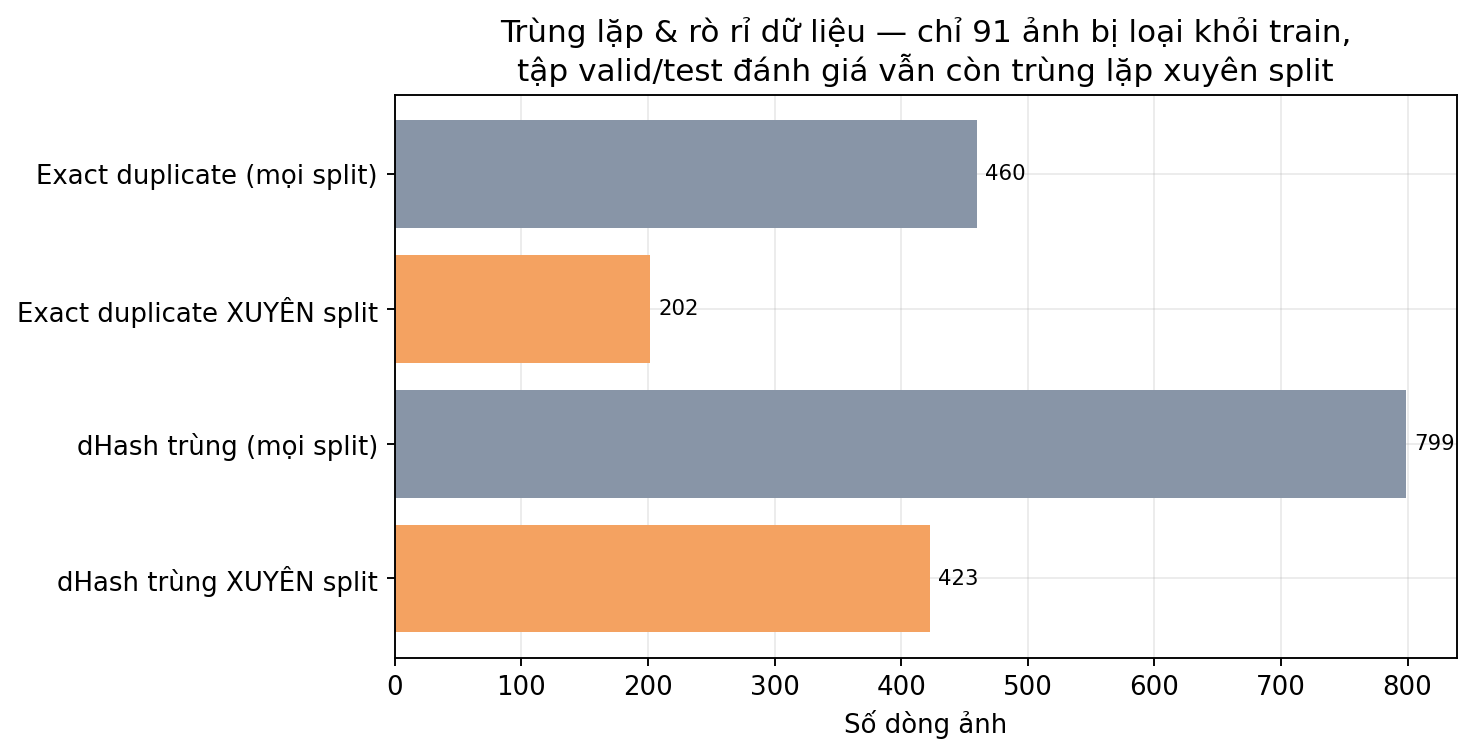
\includegraphics[width=0.82\textwidth]{figures/04_leakage.png}
\caption{Trùng lặp và rò rỉ --- chỉ 91 ảnh bị loại khỏi tập huấn luyện, valid/test vẫn còn trùng}
\label{fig:leak}
\end{figure}

\hopnhanmanh[Nhận xét CH-A]{Notebook chỉ loại 91 ảnh exact-cross-split khỏi tập huấn luyện
($3.530 \to 3.439$). Vẫn còn 202 ảnh trùng chính xác và 423 ảnh gần trùng xuyên split không bị
loại ở tập valid/test. Hệ quả: một phần điểm mAP 0,97 có thể đến từ việc mô hình đã ``thấy'' ảnh
rất giống lúc huấn luyện --- con số thực có thể thấp hơn.}

\section{CH-B --- Khoảng cách đèn tín hiệu và biển báo}

Bảng~\ref{tab:perclass} trình bày hiệu năng theo từng lớp, sắp xếp giảm dần theo mAP@0,5:0,95.

\begin{table}[H]
\centering
\caption{Hiệu năng theo lớp trên tập test}
\label{tab:perclass}
\small
\begin{tabular}{llrrrrr}
\toprule
\textbf{Lớp} & \textbf{Nhóm} & \textbf{Inst.} & \textbf{P} & \textbf{R} & \textbf{mAP@.5}
& \textbf{mAP@.5:.95} \\
\midrule
Stop & Biển báo & 50 & 0,999 & 1,000 & 0,995 & 0,899 \\
Speed Limit 80 & Biển báo & 61 & 0,977 & 1,000 & 0,995 & 0,878 \\
Speed Limit 100 & Biển báo & 46 & 0,968 & 1,000 & 0,994 & 0,871 \\
Speed Limit 70 & Biển báo & 53 & 0,922 & 0,943 & 0,973 & 0,867 \\
Speed Limit 20 & Biển báo & 46 & 0,972 & 0,978 & 0,973 & 0,866 \\
Speed Limit 120 & Biển báo & 44 & 0,930 & 1,000 & 0,985 & 0,863 \\
Speed Limit 30 & Biển báo & 60 & 0,983 & 0,966 & 0,984 & 0,860 \\
Speed Limit 60 & Biển báo & 45 & 1,000 & 0,933 & 0,992 & 0,859 \\
Speed Limit 50 & Biển báo & 50 & 0,928 & 0,960 & 0,987 & 0,856 \\
Speed Limit 40 & Biển báo & 53 & 0,977 & 0,962 & 0,982 & 0,838 \\
Speed Limit 10 & Biển báo & 3 & 1,000 & 0,971 & 0,995 & 0,830 \\
Speed Limit 90 & Biển báo & 34 & 0,995 & 0,971 & 0,993 & 0,827 \\
Speed Limit 110 & Biển báo & 21 & 0,906 & 0,905 & 0,930 & 0,784 \\
\textbf{Green Light} & \textbf{Đèn} & 110 & 0,962 & 0,921 & 0,950 & \textbf{0,576} \\
\textbf{Red Light} & \textbf{Đèn} & 94 & 0,887 & 0,755 & 0,825 & \textbf{0,506} \\
\bottomrule
\end{tabular}
\end{table}

\begin{figure}[H]
\centering
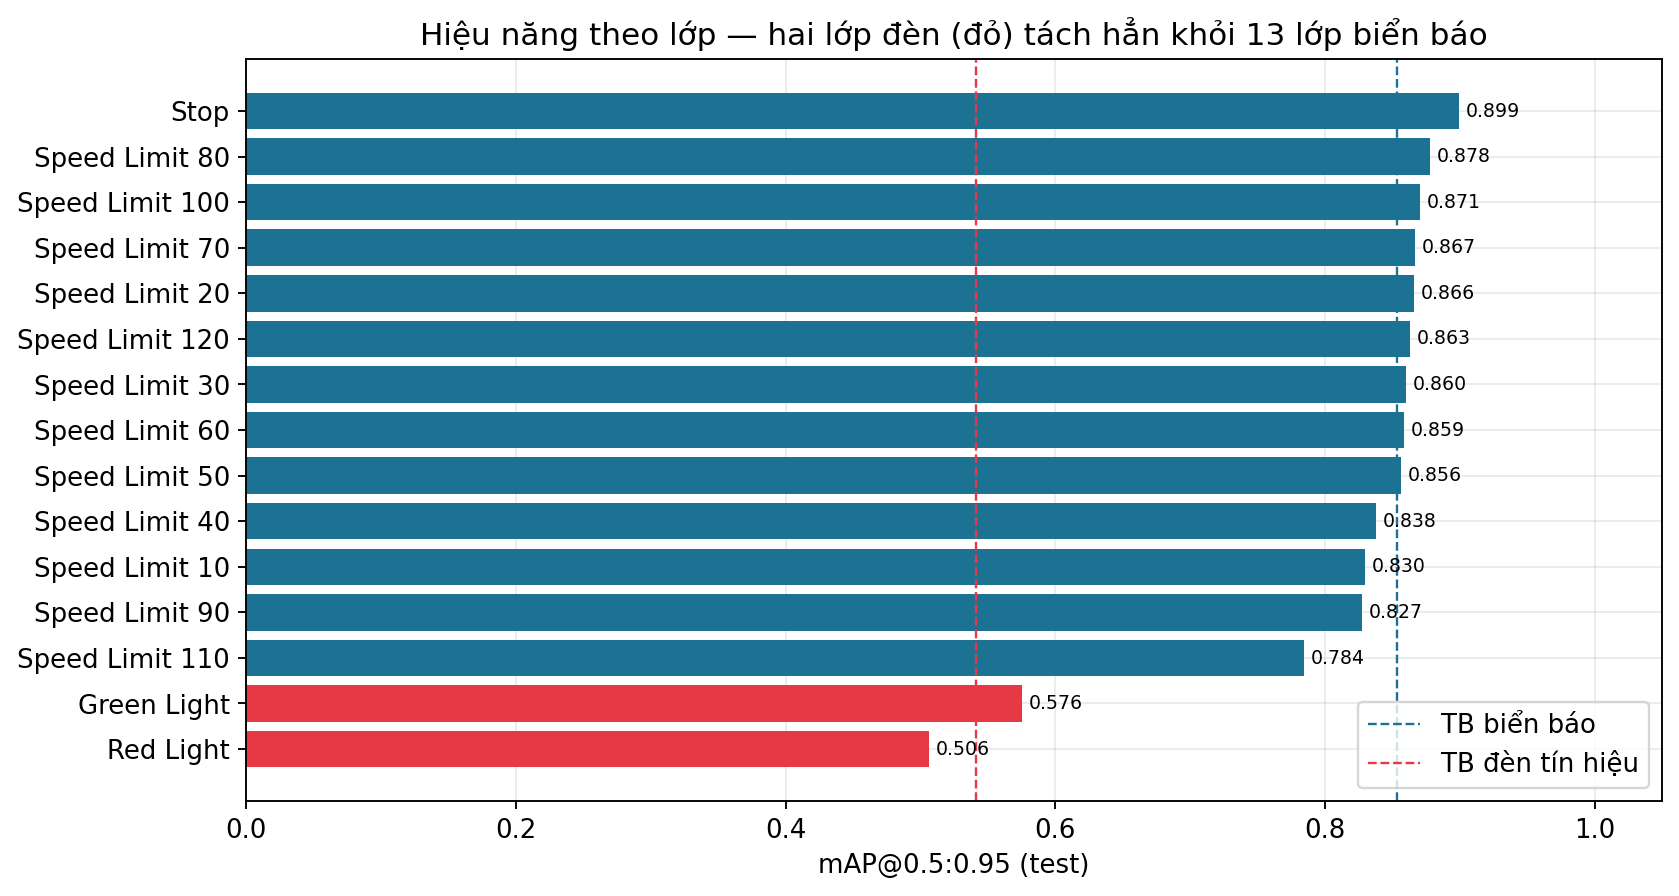
\includegraphics[width=0.92\textwidth]{figures/01_per_class_ap.png}
\caption{Hiệu năng theo lớp --- hai lớp đèn (đỏ) tách hẳn khỏi 13 lớp biển báo}
\label{fig:perclass}
\end{figure}

\begin{figure}[H]
\centering
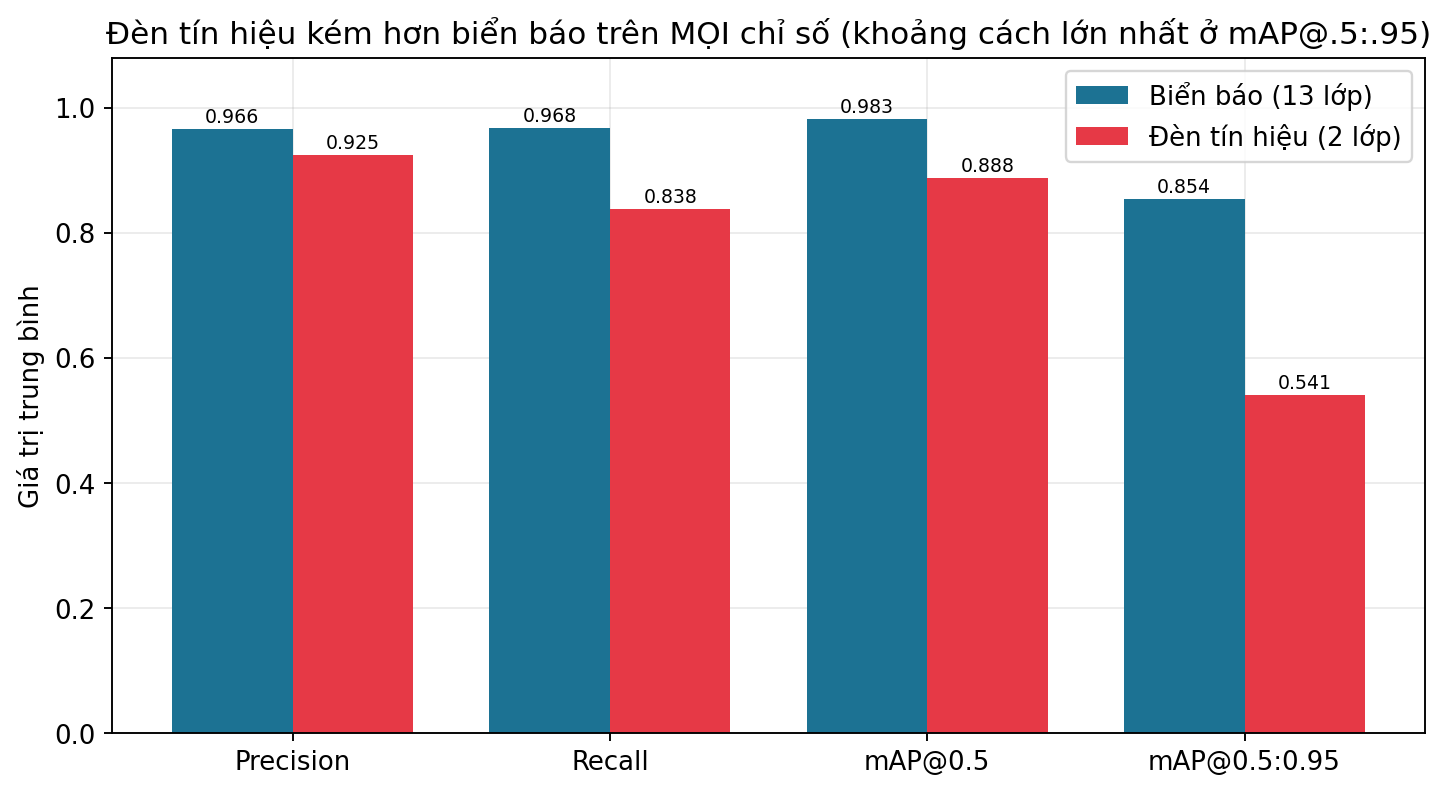
\includegraphics[width=0.82\textwidth]{figures/02_light_vs_sign.png}
\caption{Đèn tín hiệu kém hơn biển báo trên mọi chỉ số}
\label{fig:lightsign}
\end{figure}

\hopnhanmanh[Nhận xét CH-B]{Trung bình mAP@0,5:0,95: đèn tín hiệu 0,541 so với biển báo 0,854 ---
chênh 0,313. Kiểm định Mann--Whitney một phía cho $p = 0{,}0095$: khác biệt có ý nghĩa dù chỉ có
2 lớp đèn. Red Light là lớp kém nhất (mAP@0,5:0,95 = 0,506; recall chỉ 0,755).}

\section{CH-C --- Hiếm không đồng nghĩa với khó}

Một giả thuyết tự nhiên là ``đèn kém vì hiếm''. Bằng chứng bác bỏ điều này: tương quan Spearman
giữa số đối tượng trên test và mAP@0,5:0,95 là $\rho = 0{,}032$ ($p = 0{,}91$) --- gần như bằng
0 (Hình~\ref{fig:rarity}). Ngược lại, hai lớp có \emph{nhiều} đối tượng nhất trên tập test
(Green Light 110 và Red Light 94 đối tượng) lại rơi đúng vào nhóm kém nhất.

\begin{figure}[H]
\centering
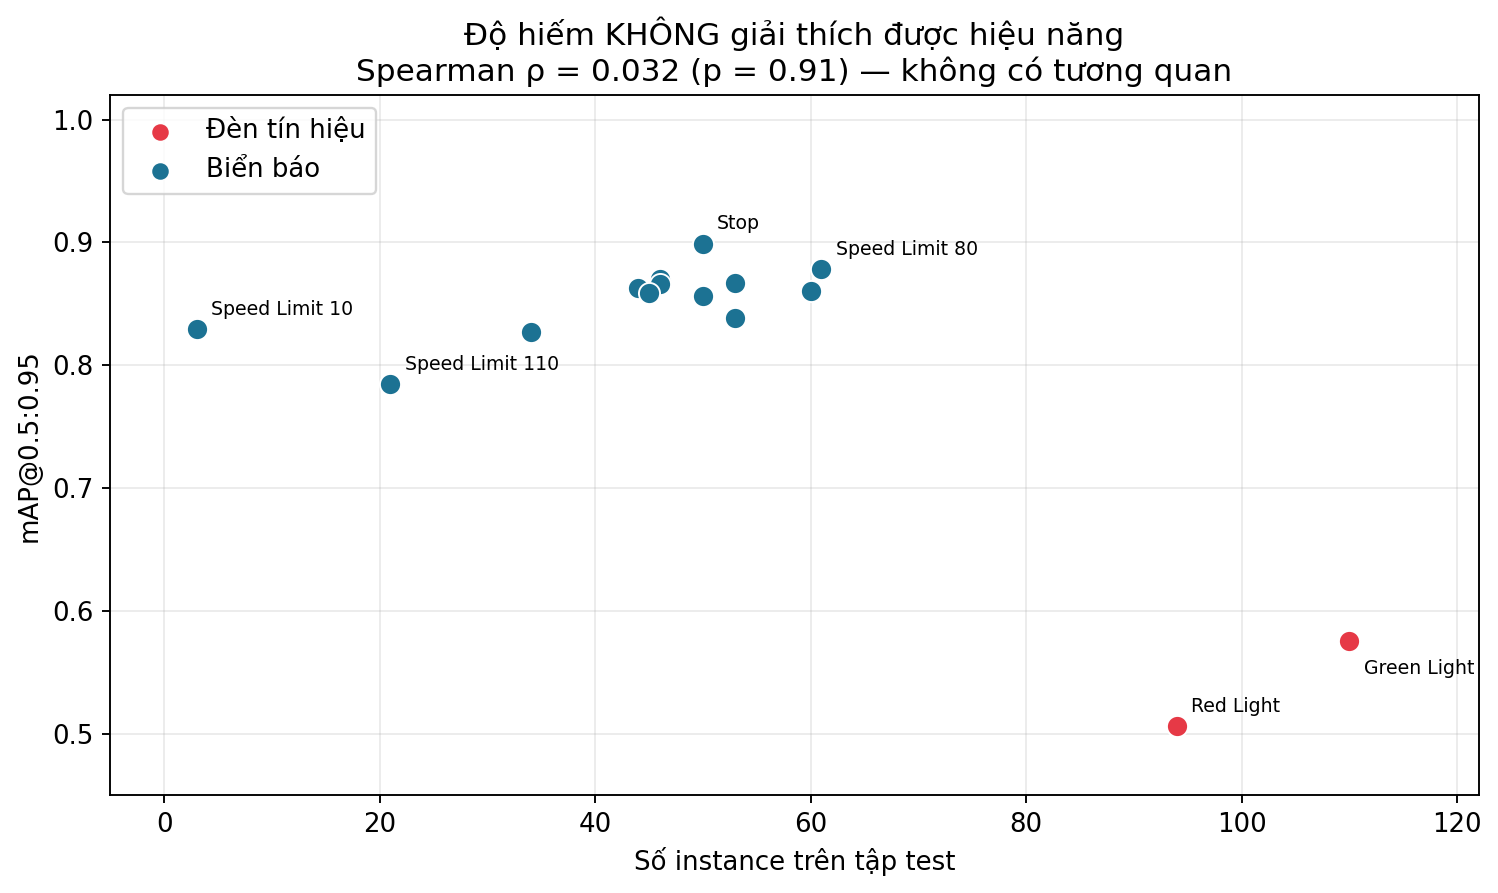
\includegraphics[width=0.82\textwidth]{figures/03_rarity_vs_ap.png}
\caption{Độ hiếm không giải thích được hiệu năng ($\rho \approx 0$)}
\label{fig:rarity}
\end{figure}

\hopnhanmanh[Nhận xét CH-C]{Độ hiếm của lớp không dự báo được hiệu năng --- mất cân bằng không
phải nguyên nhân. Nguyên nhân nằm ở bản chất vật thể: đèn tín hiệu thường nhỏ, độ tương phản
thấp, và hai màu đỏ/xanh dễ nhầm về hình học. Bối cảnh kích thước: 36,6\% đối tượng là ``nhỏ''
($<1\%$ diện tích ảnh) và 18,7\% là ``tí hon'' ($<0{,}1\%$).}

\section{Mất cân bằng và kích thước --- bối cảnh}

Toàn corpus có tỉ số mất cân bằng 35,8, entropy chuẩn hoá 0,953 và hệ số Gini 0,247 --- mất cân
bằng mức trung bình (Hình~\ref{fig:imb}). Độ dịch phân phối giữa các split rất nhỏ (Jensen--Shannon
$\le 0{,}008$ bit), nên chênh lệch hiệu năng không đến từ việc phân phối lớp khác nhau giữa các
tập. Về kích thước, tăng độ phân giải đầu vào làm giảm mạnh tỉ lệ vật thể tí hon
(Hình~\ref{fig:size}) --- cơ sở cho khuyến nghị tăng \texttt{imgsz} ở Chương~\ref{ch:tongket}.

\begin{figure}[H]
\centering
\begin{subfigure}{0.48\textwidth}
  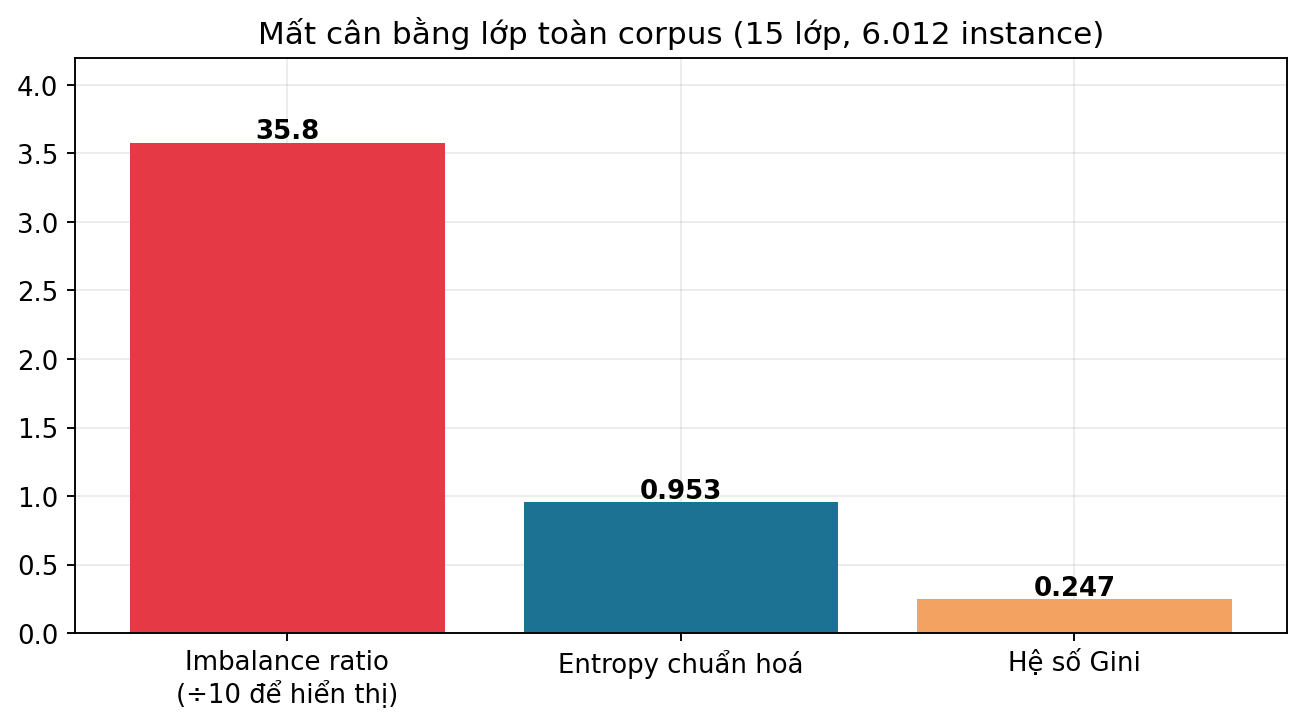
\includegraphics[width=\linewidth]{figures/05_imbalance.png}
  \caption{Mất cân bằng lớp}
  \label{fig:imb}
\end{subfigure}\hfill
\begin{subfigure}{0.48\textwidth}
  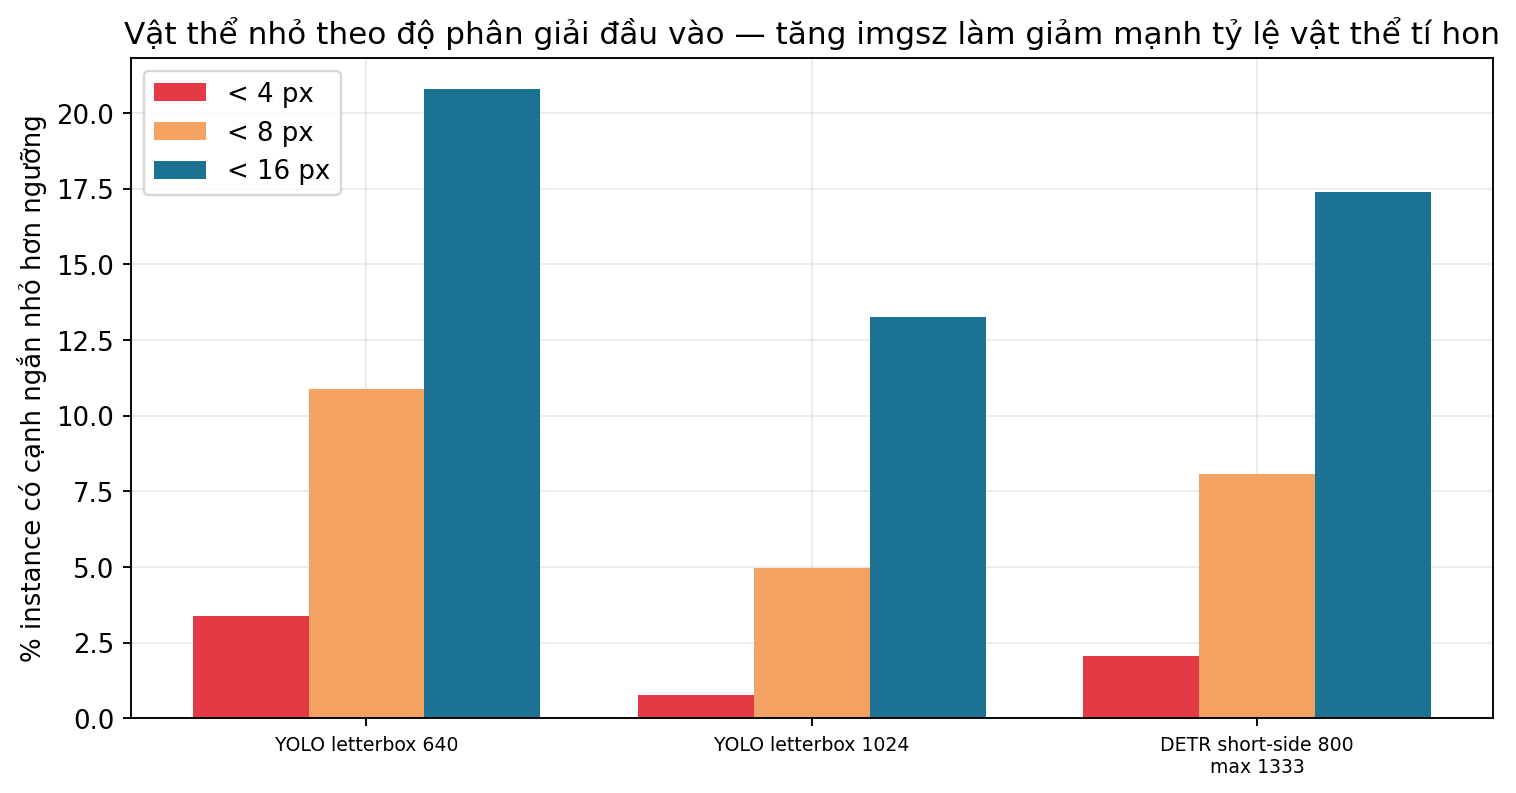
\includegraphics[width=\linewidth]{figures/06_small_objects.png}
  \caption{Vật thể nhỏ theo độ phân giải}
  \label{fig:size}
\end{subfigure}
\caption{Bối cảnh mất cân bằng (trái) và kích thước vật thể (phải)}
\label{fig:context}
\end{figure}
\clearpage
\chapter{Tổng kết}
\label{ch:tongket}

\section{Tổng hợp phát hiện}

Cả ba câu hỏi kiểm định đều chỉ về một hướng: con số mAP 0,97 cần được nhìn thận trọng hơn.
Nó có thể được data leakage nâng đỡ (CH-A), đồng thời che lấp chênh lệch lớn giữa các lớp
(CH-B), và chênh lệch đó bắt nguồn từ loại vật thể chứ không phải mất cân bằng (CH-C).

\begin{itemize}
  \item \textbf{CH-A --- Rò rỉ:} 202 ảnh trùng chính xác và 423 ảnh gần trùng xuyên split chưa
  được khử ở tập đánh giá.
  \item \textbf{CH-B --- Khoảng cách:} đèn 0,541 so với biển 0,854 (chênh 0,313; $p = 0{,}0095$).
  \item \textbf{CH-C --- Nguyên nhân:} độ hiếm không liên quan ($\rho = 0{,}032$); lỗi tập trung
  ở đèn tín hiệu.
\end{itemize}

\section{Khuyến nghị}

\begin{itemize}
  \item Khử trùng lặp xuyên split ở \emph{cả} tập valid/test trước khi báo cáo mAP; báo cáo thêm
  mAP sau khi loại near-duplicate để thấy mức chênh.
  \item Báo cáo AP theo từng lớp và theo nhóm (đèn/biển) thay vì chỉ mAP tổng, để không che giấu
  điểm yếu.
  \item Cải thiện lớp đèn tín hiệu: tăng độ phân giải đầu vào (\texttt{imgsz} 896/1024), bổ sung
  mẫu đèn khó, và phân tích ma trận nhầm lẫn đỏ$\leftrightarrow$xanh.
  \item Không dựa vào oversampling lớp hiếm để sửa lỗi đèn, vì độ hiếm không phải nguyên nhân.
\end{itemize}

\section{Hạn chế}

Đề tài ở chế độ \textit{results-only} nên không chạy lại mô hình sau khi khử rò rỉ để đo trực
tiếp mức sụt mAP; kết luận về ảnh hưởng của rò rỉ mang tính định lượng phơi nhiễm, không phải đo
can thiệp. Nhóm đèn chỉ có hai lớp nên kiểm định thống kê tuy có ý nghĩa vẫn cần thận trọng khi
khái quát.

\section{Sản phẩm kèm theo}

\begin{itemize}
  \item Pipeline phân tích tái lập (\texttt{src/}) kèm kiểm thử tự động (\texttt{pytest}, 6/6 đạt).
  \item Ứng dụng web Streamlit (\texttt{app/app.py}) trình bày toàn bộ phân tích.
  \item Báo cáo Word (\texttt{.docx}), báo cáo LaTeX (mẫu trường) và slide trình bày.
\end{itemize}
\clearpage

\phantomsection
\addcontentsline{toc}{chapter}{TÀI LIỆU THAM KHẢO}
% IEEEtran có trên Overleaf; nếu máy biên dịch thiếu, tự lùi về ieeetr (cùng kiểu số [1]).
\IfFileExists{IEEEtran.bst}{\bibliographystyle{IEEEtran}}{\bibliographystyle{ieeetr}}
% Đưa TẤT CẢ tài liệu trong references.bib vào danh mục (kể cả mục chỉ tham khảo nền tảng).
\nocite{*}
\bibliography{references}
\clearpage

\appendix
\chapter*{PHỤ LỤC}
\addcontentsline{toc}{chapter}{PHỤ LỤC}
\markboth{PHỤ LỤC}{}

Phụ lục liệt kê toàn bộ tài nguyên công khai phục vụ việc tái lập (reproducibility) kết quả đề
tài. Tất cả các URL dưới đây có thể truy cập công khai tại thời điểm nộp đề tài.

\section*{Phụ lục A: Mã nguồn (GitHub)}
\addcontentsline{toc}{section}{Phụ lục A: Mã nguồn (GitHub)}
\label{app:github}

\begin{itemize}[leftmargin=1.5cm]
\item \textbf{Thư mục dự án:} \texttt{data-analysis/traffic-yolo-analysis/}
\item \textbf{Cấu trúc thư mục quan trọng:}
\begin{itemize}
\item \texttt{data/notebook/} --- notebook Kaggle nguồn (\texttt{traffic-yolo-v2-run.ipynb})
\item \texttt{src/} --- mã trích xuất, phân tích kiểm định, vẽ hình
\item \texttt{results/tables/} --- bảng CSV trích từ output notebook
\item \texttt{results/figs/} --- hình sinh tự động
\item \texttt{app/app.py} --- ứng dụng web Streamlit
\item \texttt{tests/} --- kiểm thử tự động (pytest)
\item \texttt{reports/} --- báo cáo Word, LaTeX và slide
\end{itemize}
\end{itemize}

\section*{Phụ lục B: Bộ dữ liệu}
\addcontentsline{toc}{section}{Phụ lục B: Bộ dữ liệu}
\label{app:dataset}

\begin{itemize}[leftmargin=1.5cm]
\item \textbf{Bộ dữ liệu:} \url{https://www.kaggle.com/datasets/pkdarabi/cardetection}
\begin{itemize}
\item Quy mô: 4.969 ảnh, 6.012 đối tượng, 15 lớp (đèn tín hiệu + biển báo).
\item Notebook nguồn: \url{https://www.kaggle.com/code/tudeptraine/traffic-yolo-v2-run}
\item Ngày truy cập: tháng 7/2026.
\end{itemize}
\end{itemize}

\section*{Phụ lục C: Hướng dẫn tái lập}
\addcontentsline{toc}{section}{Phụ lục C: Hướng dẫn tái lập}
\label{app:repro}

\begin{lstlisting}[language=bash,caption={Các bước tái lập kết quả}]
# 1. Cai dat moi truong
python -m venv .venv && source .venv/bin/activate
pip install -r requirements.txt

# 2. Chay toan bo pipeline phan tich thu cap
#    (trich xuat -> kiem dinh -> ve hinh)
python -m src.run_pipeline

# 3. Kiem thu tu dong
pytest

# 4. Mo ung dung web
streamlit run app/app.py
\end{lstlisting}

\textbf{Môi trường:} Python 3, các thư viện \texttt{pandas}, \texttt{scipy}, \texttt{matplotlib};
hạt giống ngẫu nhiên \texttt{seed=42}. Số liệu gốc do notebook Kaggle sinh trên GPU Tesla T4
(Ultralytics 8.4.95). Phân tích thứ cấp chạy hoàn toàn trên CPU.


\end{document}
